% This LaTeX document needs to be compiled with XeLaTeX.
\documentclass[10pt]{article}
\usepackage[utf8]{inputenc}
\usepackage{graphicx}
\usepackage[export]{adjustbox}
\graphicspath{ {./images/} }
\usepackage{amsmath}
\usepackage{amsfonts}
\usepackage{amssymb}
\usepackage[version=4]{mhchem}
\usepackage{stmaryrd}
\usepackage[fallback]{xeCJK}
\usepackage{polyglossia}
\usepackage{fontspec}
\setCJKmainfont{Noto Serif CJK TC}

\setmainlanguage{polish}
\setmainfont{CMU Serif}

\title{ARKUSZ PRÓBNEJ MATURY Z OPERONEM MATEMATYKA \\
 POZIOM PODSTAWOWY }

\author{}
\date{}


\begin{document}
\maketitle
\section*{LISTOPAD}
2012

\section*{Czas pracy: 170 minut}
\section*{Instrukcja dla zdającego}
\begin{enumerate}
  \item Sprawdź, czy arkusz egzaminacyjny zawiera 14 stron (zadania 1.-32.). Ewentualny brak zgłoś przewodniczącemu zespołu nadzorującego egzamin.
  \item Rozwiązania zadań i odpowiedzi zapisz w miejscu na to przeznaczonym.
  \item W zadaniach zamkniętych (1.-23.) zaznacz poprawną odpowiedź.
  \item W rozwiązaniach zadań otwartych (24.-32.) przedstaw tok rozumowania prowadzący do ostatecznego wyniku.
  \item Pisz czytelnie. Używaj długopisu/pióra tylko z czarnym tuszem/atramentem.
  \item Nie używaj korektora, a błędne zapisy wyraźnie przekreśl.
  \item Zapisy w brudnopisie nie będą oceniane.
  \item Obok numeru każdego zadania podana jest maksymalna liczba punktów możliwych do uzyskania.
  \item Możesz korzystać z zestawu wzorów matematycznych, cyrkla i linijki oraz kalkulatora.
\end{enumerate}

\section*{Życzymy powodzenia!}
Wpisuje zdający przed rozpoczęciem pracy\\
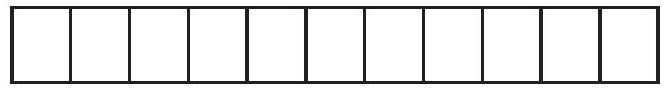
\includegraphics[max width=\textwidth, center]{2024_11_21_a38d702bc7be8115942cg-01(1)}

PESEL ZDAJĄCEGO

Za rozwiązanie wszystkich zadań można otrzymać łącznie 50 punktów.\\
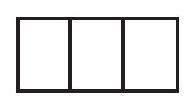
\includegraphics[max width=\textwidth, center]{2024_11_21_a38d702bc7be8115942cg-01}

KOD ZDAJĄCEGO

\section*{ZADANIA ZAMKNIĘTE}
W zadaniach od 1. do 23. wybierz i zaznacz jedną poprawną odpowiedź.

\section*{Zadanie 1. (1 pkt)}
Wartość liczby \(a=16 \sqrt[3]{4}\) jest równa wartości liczby:\\
A. \(2^{\frac{4}{3}}\)\\
B. \(2^{\frac{7}{3}}\)\\
C. \(2^{\frac{5}{3}}\)\\
D. \(2^{\frac{14}{3}}\)

\section*{Zadanie 2. (1 pkt)}
Miejscem zerowym funkcji \(f\) określonej wzorem \(f(x)=\left\{\begin{array}{ll}x^{2}-1 & \text { dla } x \in(-\infty,-4\rangle \\ 5 x+10 & \text { dla } x \in(-4,2) \\ x+4 & \text { dla } x \in\langle 2,+\infty)\end{array}\right.\) jest:\\
A. -4\\
B. -2\\
C. -1\\
D. 1

\section*{Zadanie 3. (1 pkt)}
Funkcja \(f\), określona wzorem \(f(x)=x^{2}-3 x-4\), przyjmuje wartości ujemne jedynie w przedziale:\\
A. \(\left(-\infty, \frac{3}{2}\right)\)\\
B. \((-\infty,-1) \cup(4,+\infty)\)\\
C. \((-1,4)\)\\
D. \((-4,1)\)

Zadanie 4. (1 pkt)\\
Wartość liczby \(25^{\log _{5} 2}\) jest równa:\\
A. 2\\
B. 4\\
C. 5\\
D. \(2^{5}\)

\section*{Zadanie 5. (1 pkt)}
Dany jest ciąg \(\left(a_{n}\right)\) o wyrazie ogólnym \(a_{n}=-n^{2}+16\) dla \(n \geq 1\). Liczba dodatnich wyrazów tego ciągu jest równa:\\
A. 3\\
B. 4\\
C. 5\\
D. 7

\section*{Zadanie 6. (1 pkt)}
Kwotę \(10000 \mathrm{zł}\) wpłacamy do banku na 4 lata. Kapitalizacja odsetek jest dokonywana w tym banku co kwartał, a roczna stopa procentowa wynosi \(3 \%\). Po 4 latach kwotę na rachunku będzie można opisać wzorem:\\
A. \(10000 \cdot(1,0075)^{4}\)\\
B. \(10000 \cdot(1,03)^{4}\)\\
C. \(10000 \cdot(1,03)^{16}\)\\
D. \(10000 \cdot(1,0075)^{16}\)

\section*{Zadanie 7. (1 pkt)}
Dane liczby: \(x=\frac{3}{\sqrt{5}-2}, y=\frac{12}{\sqrt{5}-1}+1, z=3 \sqrt{5}+2\) tworzą rosnący ciąg arytmetyczny w ko-\\
lejności:\\
A. \(z, y, x\)\\
B. \(y, x, z\)\\
C. \(x, y, z\)\\
D. \(z, x, y\)

\section*{BRUDNOPIS (nie podlega ocenie)}
\begin{center}

\includegraphics[max width=\textwidth]{2024_11_21_a38d702bc7be8115942cg-03}
\end{center}

\section*{Zadanie 8. (1 pkt)}
Suma \(2 n\) początkowych liczb naturalnych dodatnich parzystych jest równa:\\
A. \(S_{2 n}=8 n^{2}+4 n\)\\
B. \(S_{2 n}=4 n^{2}+2 n\)\\
C. \(S_{2 n}=4 n^{2}+n\)\\
D. \(S_{2 n}=2 n^{2}+2 n\)

\section*{Zadanie 9. (1 pkt)}
W trójkącie równoramiennym wysokość jest dwa razy dłuższa od podstawy. Wynika stąd, że sinus kąta przy podstawie wynosi:\\
A. \(\frac{\sqrt{17}}{17}\)\\
B. \(\frac{\sqrt{5}}{5}\)\\
C. \(\frac{4 \sqrt{17}}{17}\)\\
D. \(\frac{1}{17}\)

\section*{Zadanie 10. (1 pkt)}
Dziedziną funkcji \(f\), określonej wzorem \(f(x)=\frac{x-5}{x^{2}+4}\), jest zbiór:\\
A. \(\boldsymbol{R} \backslash\{-4,4\}\)\\
B. \(\boldsymbol{R} \backslash\{-4\}\)\\
C. \(\boldsymbol{R}\)\\
D. \(\boldsymbol{R} \backslash\{5\}\)

\section*{Zadanie 11. (1 pkt)}
Liczbą przeciwną do liczby \(a=5^{\frac{2}{3}}\) jest:\\
A. \(5^{\frac{3}{2}}\)\\
B. \(-5^{\frac{3}{2}}\)\\
C. \(5^{-\frac{2}{3}}\)\\
D. \(-5^{\frac{2}{3}}\)

\section*{Zadanie 12. (1 pkt)}
Wzór funkcji, której wykres powstaje przez przesunięcie wykresu funkcji \(f\) o 10 jednostek w dót, to:\\
A. \(y=f(x+10)\)\\
B. \(y=f(x)+10\)\\
C. \(y=f(x-10)\)\\
D. \(y=f(x)-10\)

\section*{Zadanie 13. (1 pkt)}
Rzucono sześcienną kostką do gry. Prawdopodobieństwo, że wyrzucona liczba oczek jest liczbą pierwszą, wynosi:\\
A. \(\frac{4}{6}\)\\
B. \(\frac{3}{6}\)\\
C. \(\frac{2}{6}\)\\
D. \(\frac{1}{6}\)

\section*{Zadanie 14. (1 pkt)}
Kąt \(\alpha\) jest ostry i \(\operatorname{tg} \alpha=\frac{12}{5}\). Wówczas \(\cos \alpha\) jest równy:\\
A. \(\frac{5}{12}\)\\
B. \(\frac{5}{13}\)\\
C. \(\frac{10}{13}\)\\
D. \(\frac{12}{13}\)

\section*{Zadanie 15. (1 pkt)}
Wielomian \(W=x^{3}-2 x^{2}-4 x+8\) po rozłożeniu na czynniki ma postać wyrażenia:\\
A. \(x^{2}(x-2)\)\\
B. \(x^{2}(x-4)\)\\
C. \((x+2)(x-2)^{2}\)\\
D. \((x-2)(x+2)^{2}\)

\section*{BRUDNOPIS (nie podlega ocenie)}
\begin{center}

\includegraphics[max width=\textwidth]{2024_11_21_a38d702bc7be8115942cg-05}
\end{center}

\section*{Zadanie 16. (1 pkt)}
Zbiór \((-\infty,-8\rangle \cup\langle-4,+\infty)\) jest rozwiązaniem nierówności:\\
A. \(|x-6| \leq 2\)\\
B. \(|x-6| \geq 2\)\\
C. \(|x+6| \leq 2\)\\
D. \(|x+6| \geq 2\)

\section*{Zadanie 17. (1 pkt)}
Funkcja \(f(x)=2 x^{2}-4 x+5\) jest malejąca w przedziale:\\
A. \((2,+\infty)\)\\
B. \((-\infty, 2)\)\\
C. \((-\infty, 1)\)\\
D. \((1,+\infty)\)

\section*{Zadanie 18. (1 pkt)}
Proste \(l\) i \(k\) są prostopadłe i \(l: 2 x-9 y+6=0, k: y=a x+b\). Wówczas:\\
A. \(a=-\frac{2}{9}\)\\
B. \(a=\frac{2}{9}\)\\
C. \(a=-\frac{9}{2}\)\\
D. \(a=\frac{9}{2}\)

\section*{Zadanie 19. (1 pkt)}
Iloraz ciągu geometrycznego o wyrazie ogólnym \(a_{n}=2 \cdot 7^{n}\) jest równy:\\
A. \(q=2\)\\
B. \(q=7\)\\
C. \(q=9\)\\
D. \(q=28\)

Zadanie 20. (1 pkt)\\
Równanie \((x+6)^{2}+y^{2}=4\) opisuje okrąg o środku w punkcie \(S\) i promieniu \(r\). Wówczas:\\
A. \(S=(-6,0), r=4\)\\
B. \(S=(6,0), r=4\)\\
C. \(S=(6,0), r=2\)\\
D. \(S=(-6,0), r=2\)

\section*{Zadanie 21. (1 pkt)}
Długość promienia \(r\) okręgu opisanego na kwadracie jest równa \(2 \sqrt{3}\). Długość boku tego kwadratu ma wartość:\\
A. \(4 \sqrt{3}\)\\
B. \(2 \sqrt{6}\)\\
C. \(4 \sqrt{6}\)\\
D. \(2 \sqrt{5}\)

\section*{Zadanie 22. (1 pkt)}
W turnieju szachowym, rozgrywanym systemem każdy z każdym, bez rewanżu, miało brać udział 8 zawodników. Jeden z nich zrezygnował. Liczba zaplanowanych rozgrywek zmniejszyła się o:\\
A. 1\\
B. 14\\
C. 7\\
D. 8

\section*{Zadanie 23. (1 pkt)}
Proste \(l\) i \(k\) są równoległe oraz \(|O A|=6,|A B|=10,|O C|=48\). Odcinek \(O D\) ma długość:\\
A. 12\\
B. 18\\
C. \(\frac{18}{5}\)\\
D. \(\frac{144}{5}\)\\
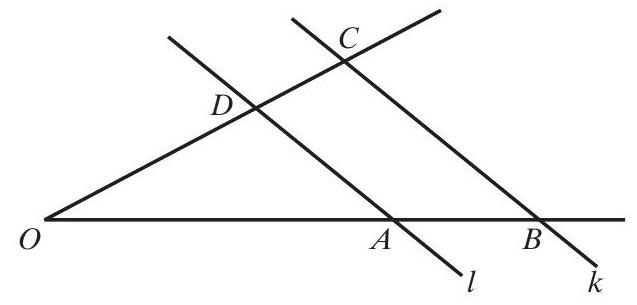
\includegraphics[max width=\textwidth, center]{2024_11_21_a38d702bc7be8115942cg-06}

\section*{BRUDNOPIS (nie podlega ocenie)}
\begin{center}

\includegraphics[max width=\textwidth]{2024_11_21_a38d702bc7be8115942cg-07}
\end{center}

\section*{ZADANIA OTWARTE}
\section*{Rozwiązania zadań o numerach od 24. do 32. należy zapisać}
w wyznaczonych miejscach pod treścią zadania.

\section*{Zadanie 24. (2 pkt)}
W ciągu arytmetycznym \(\left(a_{n}\right)\) drugi wyraz jest równy 7 , a szósty 17 . Wyznacz pierwszy wyraz i różnicę tego ciągu.\\

\includegraphics[max width=\textwidth, center]{2024_11_21_a38d702bc7be8115942cg-08}

Odpowiedź:

\section*{Zadanie 25. (2 pkt)}
Średni wzrost sportowców w drużynie siatkarskiej, liczącej 6 chłopców, wynosił 174 cm . Po przyjęciu do zespołu dwóch braci o tej samej wysokości średnia wzrostu zwiększyła się o \(0,5 \mathrm{~cm}\). Oblicz, jak wysocy są bracia.\\

\includegraphics[max width=\textwidth, center]{2024_11_21_a38d702bc7be8115942cg-08(1)}

Odpowiedź:

Zadanie 26. (2 pkt)\\
Rozwiąż równanie \(2 x^{3}+8 x^{2}-3 x-12=0\).

\begin{center}
\begin{tabular}{|c|c|c|c|c|c|c|c|c|c|c|c|c|c|c|c|c|c|c|c|c|c|c|c|}
\hline
 &  &  &  &  &  &  &  &  &  &  &  &  &  &  &  &  &  &  &  &  &  &  &  \\
\hline
 &  &  &  &  &  &  &  &  &  &  &  &  &  &  &  &  &  &  &  &  &  &  &  \\
\hline
 &  &  &  &  &  &  &  &  &  &  &  &  &  &  &  &  &  &  &  &  &  &  &  \\
\hline
 &  &  &  &  &  &  &  &  &  &  &  &  &  &  &  &  &  &  &  &  &  &  &  \\
\hline
 &  &  &  &  &  &  &  &  &  &  &  &  &  &  &  &  &  &  &  &  &  &  &  \\
\hline
 &  &  &  &  &  &  &  &  &  &  &  &  &  &  &  &  &  &  &  &  &  &  &  \\
\hline
 &  &  &  &  &  &  &  &  &  &  &  &  &  &  &  &  &  &  &  &  &  &  &  \\
\hline
 &  &  &  &  &  &  &  &  &  &  &  &  &  &  &  &  &  &  &  &  &  &  &  \\
\hline
 &  &  &  &  &  &  &  &  &  &  &  &  &  &  &  &  &  &  &  &  &  &  &  \\
\hline
 &  &  &  &  &  &  &  &  &  &  &  &  &  &  &  &  &  &  &  &  &  &  &  \\
\hline
 &  &  &  &  &  &  &  &  &  &  &  &  &  &  &  &  &  &  &  &  &  &  &  \\
\hline
 &  &  &  &  &  &  &  &  &  &  &  &  &  &  &  &  &  &  &  &  &  &  &  \\
\hline
 &  &  &  &  &  &  &  &  &  &  &  &  &  &  &  &  &  &  &  &  &  &  &  \\
\hline
 &  &  &  &  &  &  &  &  &  &  &  &  &  &  &  &  &  &  &  &  &  &  &  \\
\hline
 &  &  &  &  &  &  &  &  &  &  &  &  &  &  &  &  &  &  &  &  &  &  &  \\
\hline
 &  &  &  &  &  &  &  &  &  &  &  &  &  &  &  &  &  &  &  &  &  &  &  \\
\hline
 &  &  &  &  &  &  &  &  &  &  &  &  &  &  &  &  &  &  &  &  &  &  &  \\
\hline
\end{tabular}
\end{center}

Odpowiedź: \(\qquad\)

\section*{Zadanie 27. (2 pkt)}
Rozwiąż nierówność \(x^{2}-9>0\).

\begin{center}
\begin{tabular}{|c|c|c|c|c|c|c|c|c|c|c|c|c|c|c|c|c|c|c|c|c|c|}
\hline
 &  &  &  &  &  &  &  &  &  &  &  &  &  &  &  &  &  &  &  &  &  \\
\hline
 &  &  &  &  &  &  &  &  &  &  &  &  &  &  &  &  &  &  &  &  &  \\
\hline
 &  &  &  &  &  &  &  &  &  &  &  &  &  &  &  &  &  &  &  &  &  \\
\hline
 &  &  &  &  &  &  &  &  &  &  &  &  &  &  &  &  &  &  &  &  &  \\
\hline
 &  &  &  &  &  &  &  &  &  &  &  &  &  &  &  &  &  &  &  &  &  \\
\hline
 &  &  &  &  &  &  &  &  &  &  &  &  &  &  &  &  &  &  &  &  &  \\
\hline
 &  &  &  &  &  &  &  &  &  &  &  &  &  &  &  &  &  &  &  &  &  \\
\hline
 &  &  &  &  &  &  &  &  &  &  &  &  &  &  &  &  &  &  &  &  &  \\
\hline
 &  &  &  &  &  &  &  &  &  &  &  &  &  &  &  &  &  &  &  &  &  \\
\hline
 &  &  &  &  &  &  &  &  &  &  &  &  &  &  &  &  &  &  &  &  &  \\
\hline
 &  &  &  &  &  &  &  &  &  &  &  &  &  &  &  &  &  &  &  &  &  \\
\hline
 &  &  &  &  &  &  &  &  &  &  &  &  &  &  &  &  &  &  &  &  &  \\
\hline
 &  &  &  &  &  &  &  &  &  &  &  &  &  &  &  &  &  &  &  &  &  \\
\hline
 &  &  &  &  &  &  &  &  &  &  &  &  &  &  &  &  &  &  &  &  &  \\
\hline
 &  &  &  &  &  &  &  &  &  &  &  &  &  &  &  &  &  &  &  &  &  \\
\hline
 &  &  &  &  &  &  &  &  &  &  &  &  &  &  &  &  &  &  &  &  &  \\
\hline
 &  &  &  &  &  &  &  &  &  &  &  &  &  &  &  &  &  &  &  &  &  \\
\hline
 &  &  &  &  &  &  &  &  &  &  &  &  &  &  &  &  &  &  &  &  &  \\
\hline
\end{tabular}
\end{center}

Odpowiedź: \(\qquad\)

\section*{Zadanie 28. (2 pkt)}
Dana jest liczba \(a=\sqrt{(2-2 \sqrt{5})^{2}}-2 \sqrt{5}\). Wykaż, że liczba \(a\) jest całkowita.\\

\includegraphics[max width=\textwidth, center]{2024_11_21_a38d702bc7be8115942cg-10}

Odpowiedź:

\section*{Zadanie 29. (2 pkt)}
Długość krawędzi sześcianu zwiększono o 20\%. Oblicz, o ile procent wzrosła objętość tego sześcianu.

\begin{center}
\begin{tabular}{|c|c|c|c|c|c|c|c|c|c|c|c|c|c|c|c|c|c|c|c|c|c|c|}
\hline
 &  &  &  &  &  &  &  &  &  &  &  &  & 到 &  &  &  &  &  &  &  &  &  \\
\hline
 &  &  &  &  &  &  &  &  &  &  &  &  &  &  &  &  &  &  &  &  &  &  \\
\hline
 &  &  &  &  &  &  &  &  &  &  &  &  &  &  &  &  &  &  &  &  &  &  \\
\hline
 &  &  &  &  &  &  &  &  &  &  &  &  &  &  &  &  &  &  &  &  &  &  \\
\hline
 &  &  &  &  &  &  &  &  &  &  &  &  &  &  &  &  &  &  &  &  &  &  \\
\hline
 &  &  &  &  &  &  &  &  &  &  &  &  &  &  &  &  &  &  &  &  &  &  \\
\hline
 &  &  &  &  &  &  &  &  &  &  &  &  &  &  &  &  &  &  &  &  &  &  \\
\hline
 &  &  &  &  &  &  &  &  &  &  &  &  &  &  &  &  &  &  &  &  &  &  \\
\hline
 &  &  &  &  &  &  &  &  &  &  &  &  &  &  &  &  &  &  &  &  &  &  \\
\hline
 &  &  &  &  &  &  &  &  &  &  &  &  &  &  &  &  &  &  &  &  &  &  \\
\hline
 &  &  &  &  &  &  &  &  &  &  &  &  &  &  &  &  &  &  &  &  &  &  \\
\hline
 &  &  &  &  &  &  &  &  &  &  &  &  &  &  &  &  &  &  &  &  &  &  \\
\hline
 &  &  &  &  &  &  &  &  &  &  &  &  &  &  &  &  &  &  &  &  &  &  \\
\hline
 &  &  &  &  &  &  &  &  &  &  &  &  &  &  &  &  &  &  &  &  &  &  \\
\hline
 &  &  &  &  &  &  &  &  &  &  &  &  &  &  &  &  &  &  &  &  &  &  \\
\hline
 &  &  &  &  &  &  &  &  &  &  &  &  &  &  &  &  &  &  &  &  &  &  \\
\hline
 &  &  &  &  &  &  &  &  &  &  &  &  &  &  &  &  &  &  &  &  &  &  \\
\hline
\end{tabular}
\end{center}

\(\qquad\)

\section*{Zadanie 30. (5 pkt)}
Prosta \(y=x+4\) przecina okrąg o równaniu \((x+1)^{2}+(y-2)^{2}=25 \mathrm{w}\) punktach \(A\) i \(B\). Oblicz współrzędne punktów \(A\) i \(B\), a następnie oblicz obwód trójkąta \(A B S\), gdzie \(S\) jest środkiem danego okręgu.

\begin{center}
\begin{tabular}{|c|c|c|c|c|c|c|c|c|c|c|c|c|c|c|c|c|c|c|c|c|}
\hline
 &  &  &  &  &  &  &  &  &  &  &  &  &  &  &  &  &  &  &  &  \\
\hline
 &  &  &  &  &  &  &  &  &  &  &  &  &  &  &  &  &  &  &  &  \\
\hline
 &  &  &  &  &  &  &  &  &  &  &  &  &  &  &  &  &  &  &  &  \\
\hline
 &  &  &  &  &  &  &  &  &  &  &  &  &  &  &  &  &  &  &  &  \\
\hline
 &  &  &  &  &  &  &  &  &  &  &  &  &  &  &  &  &  &  &  &  \\
\hline
 &  &  &  &  &  &  &  &  &  &  &  &  &  &  &  &  &  &  &  &  \\
\hline
 &  &  &  &  &  &  &  &  &  &  &  &  &  &  &  &  &  &  &  &  \\
\hline
 &  &  &  &  &  &  &  &  &  &  &  &  &  &  &  &  &  &  &  &  \\
\hline
 &  &  &  &  &  &  &  &  &  &  &  &  &  &  &  &  &  &  &  &  \\
\hline
 &  &  &  &  &  &  &  &  &  &  &  &  &  &  &  &  &  &  &  &  \\
\hline
 &  &  &  &  &  &  &  &  &  &  &  &  &  &  &  &  &  &  &  &  \\
\hline
 &  &  &  &  &  &  &  &  &  &  &  &  &  &  &  &  &  &  &  &  \\
\hline
 &  &  &  &  &  &  &  &  &  &  &  &  &  &  &  &  &  &  &  &  \\
\hline
 &  &  &  &  &  &  &  &  &  &  &  &  &  &  &  &  &  &  &  &  \\
\hline
 &  &  &  &  &  &  &  &  &  &  &  &  &  &  &  &  &  &  &  &  \\
\hline
 &  &  &  &  &  &  &  &  &  &  &  &  &  &  &  &  &  &  &  &  \\
\hline
 &  &  &  &  &  &  &  &  &  &  &  &  &  &  &  &  &  &  &  &  \\
\hline
 &  &  &  &  &  &  &  &  &  &  &  &  &  &  &  &  &  &  &  &  \\
\hline
 &  &  &  &  &  &  &  &  &  &  &  &  &  &  &  &  &  &  &  &  \\
\hline
 &  &  &  &  &  &  &  &  &  &  &  &  &  &  &  &  &  &  &  &  \\
\hline
 &  &  &  &  &  &  &  &  &  &  &  &  &  &  &  &  &  &  &  &  \\
\hline
 &  &  &  &  &  &  &  &  &  &  &  &  &  &  &  &  &  &  &  &  \\
\hline
 &  &  &  &  &  &  &  &  &  &  &  &  &  &  &  &  &  &  &  &  \\
\hline
 &  &  &  &  &  &  &  &  &  &  &  &  &  &  &  &  &  &  &  &  \\
\hline
 &  &  &  &  &  &  &  &  &  &  &  &  &  &  &  &  &  &  &  &  \\
\hline
 &  &  &  &  &  &  &  &  &  &  &  &  &  &  &  &  &  &  &  &  \\
\hline
 &  &  &  &  &  &  &  &  &  &  &  &  &  &  &  &  &  &  &  &  \\
\hline
 &  &  &  &  &  &  &  &  &  &  &  &  &  &  &  &  &  &  &  &  \\
\hline
 &  &  &  &  &  &  &  &  &  &  &  &  &  &  &  &  &  &  &  &  \\
\hline
 &  &  &  &  &  &  &  &  &  &  &  &  &  &  &  &  &  &  &  &  \\
\hline
 &  &  &  &  &  &  &  &  &  &  &  &  &  &  &  &  &  &  &  &  \\
\hline
 &  &  &  &  &  &  &  &  &  &  &  &  &  &  &  &  &  &  &  &  \\
\hline
 &  &  &  &  &  &  &  &  &  &  &  &  &  &  &  &  &  &  &  &  \\
\hline
 &  &  &  &  &  &  &  &  &  &  &  &  &  &  &  &  &  &  &  &  \\
\hline
 &  &  &  &  &  &  &  &  &  &  &  &  &  &  &  &  &  &  &  &  \\
\hline
 &  &  &  &  &  &  &  &  &  &  &  &  &  &  &  &  &  &  &  &  \\
\hline
 &  &  &  &  &  &  &  &  &  &  &  &  &  &  &  &  &  &  &  &  \\
\hline
 &  &  &  &  &  &  &  &  &  &  &  &  &  &  &  &  &  &  &  &  \\
\hline
 &  &  &  &  &  &  &  &  &  &  &  &  &  &  &  &  &  &  &  &  \\
\hline
 &  &  &  &  &  &  &  &  &  &  &  &  &  &  &  &  &  &  &  &  \\
\hline
\end{tabular}
\end{center}

\section*{Zadanie 31. (5 pkt)}
Dany jest ostrosłup prawidłowy trójkątny. Pole powierzchni bocznej tego ostrosłupa jest równe 24 , a kąt płaski ściany bocznej przy podstawie ma miarę \(\alpha \mathrm{i} \operatorname{tg} \alpha=2\). Wyznacz cosinus kąta nachylenia ściany bocznej ostrosłupa do płaszczyzny jego podstawy.\\

\includegraphics[max width=\textwidth, center]{2024_11_21_a38d702bc7be8115942cg-12}

Odpowiedź:

\section*{Zadanie 32. (5 pkt)}
Turysta pokonał pieszo trasę długości 30 km z miejscowości \(A\) do miejscowości \(B\) ze stałą prędkością. Rowerem poruszałby się z prędkością o \(9 \mathrm{~km} / \mathrm{h}\) większą i przybyłby do celu o 3 godziny wcześniej. Wyznacz prędkość marszu turysty i czas przejścia tej drogi.\\

\includegraphics[max width=\textwidth, center]{2024_11_21_a38d702bc7be8115942cg-13}

Odpowiedź:

\section*{BRUDNOPIS (nie podlega ocenie)}
\begin{center}

\includegraphics[max width=\textwidth]{2024_11_21_a38d702bc7be8115942cg-14}
\end{center}


\end{document}